\documentclass[aspectratio=169]{beamer}
\mode<presentation>
\usetheme{Hannover}
\useoutertheme{sidebar}
\usecolortheme{dolphin}

\usepackage{amsmath}
\usepackage{amssymb}
\usepackage{enumerate}

%some bold math symbosl
\newcommand{\Cov}{\mathrm{Cov}}
\newcommand{\Var}{\mathrm{Var}}
\newcommand{\brho}{\boldsymbol{\rho}}
\newcommand{\bSigma}{\boldsymbol{\Sigma}}
\newcommand{\btheta}{\boldsymbol{\theta}}
\newcommand{\bbeta}{\boldsymbol{\beta}}
\newcommand{\bmu}{\boldsymbol{\mu}}
\newcommand{\bW}{\mathbf{W}}
\newcommand{\one}{\mathbf{1}}
\newcommand{\bH}{\mathbf{H}}
\newcommand{\by}{\mathbf{y}}
\newcommand{\bolde}{\mathbf{e}}
\newcommand{\bx}{\mathbf{x}}

\newcommand{\cpp}[1]{\texttt{#1}}



\title{Mathematical Biostatistics Boot Camp: Lecture 3, Expectations}

\author{Brian Caffo}
\date{\today}
\institute[Department of Biostatistics]{
  Department of Biostatistics \\
  Johns Hopkins Bloomberg School of Public Health\\
  Johns Hopkins University
}


\begin{document}

\frame{\titlepage}

\frame{
  \frametitle{Table of contents}
  \tableofcontents
}


\section{Outline}
\frame{
  \frametitle{Outline}
  \begin{enumerate}
  \item Define expected values
  \item Properties of expected values
  \item Unbiasedness of the sample mean
  \item Define variances 
  \item Define the standard deviation
  \item Calculate Bernoulli variance
  \end{enumerate}
}

\section{Expected values}
\subsection{Discrete random variables}
\begin{frame}
  \frametitle{Expected values}
  \begin{itemize}
  \item The {\bf expected value} or {\bf mean} of a random variable is the center of its
    distribution
  \item For discrete random variable $X$ with PMF $p(x)$, it is defined as follows
    $$
    E[X] = \sum_x xp(x).
    $$
    where the sum is taken over the possible values of $x$
  \item $E[X]$ represents the center of mass of a collection of
    locations and weights, $\{x, p(x)\}$
  \end{itemize}
\end{frame}


\begin{frame}
  \frametitle{Example}
  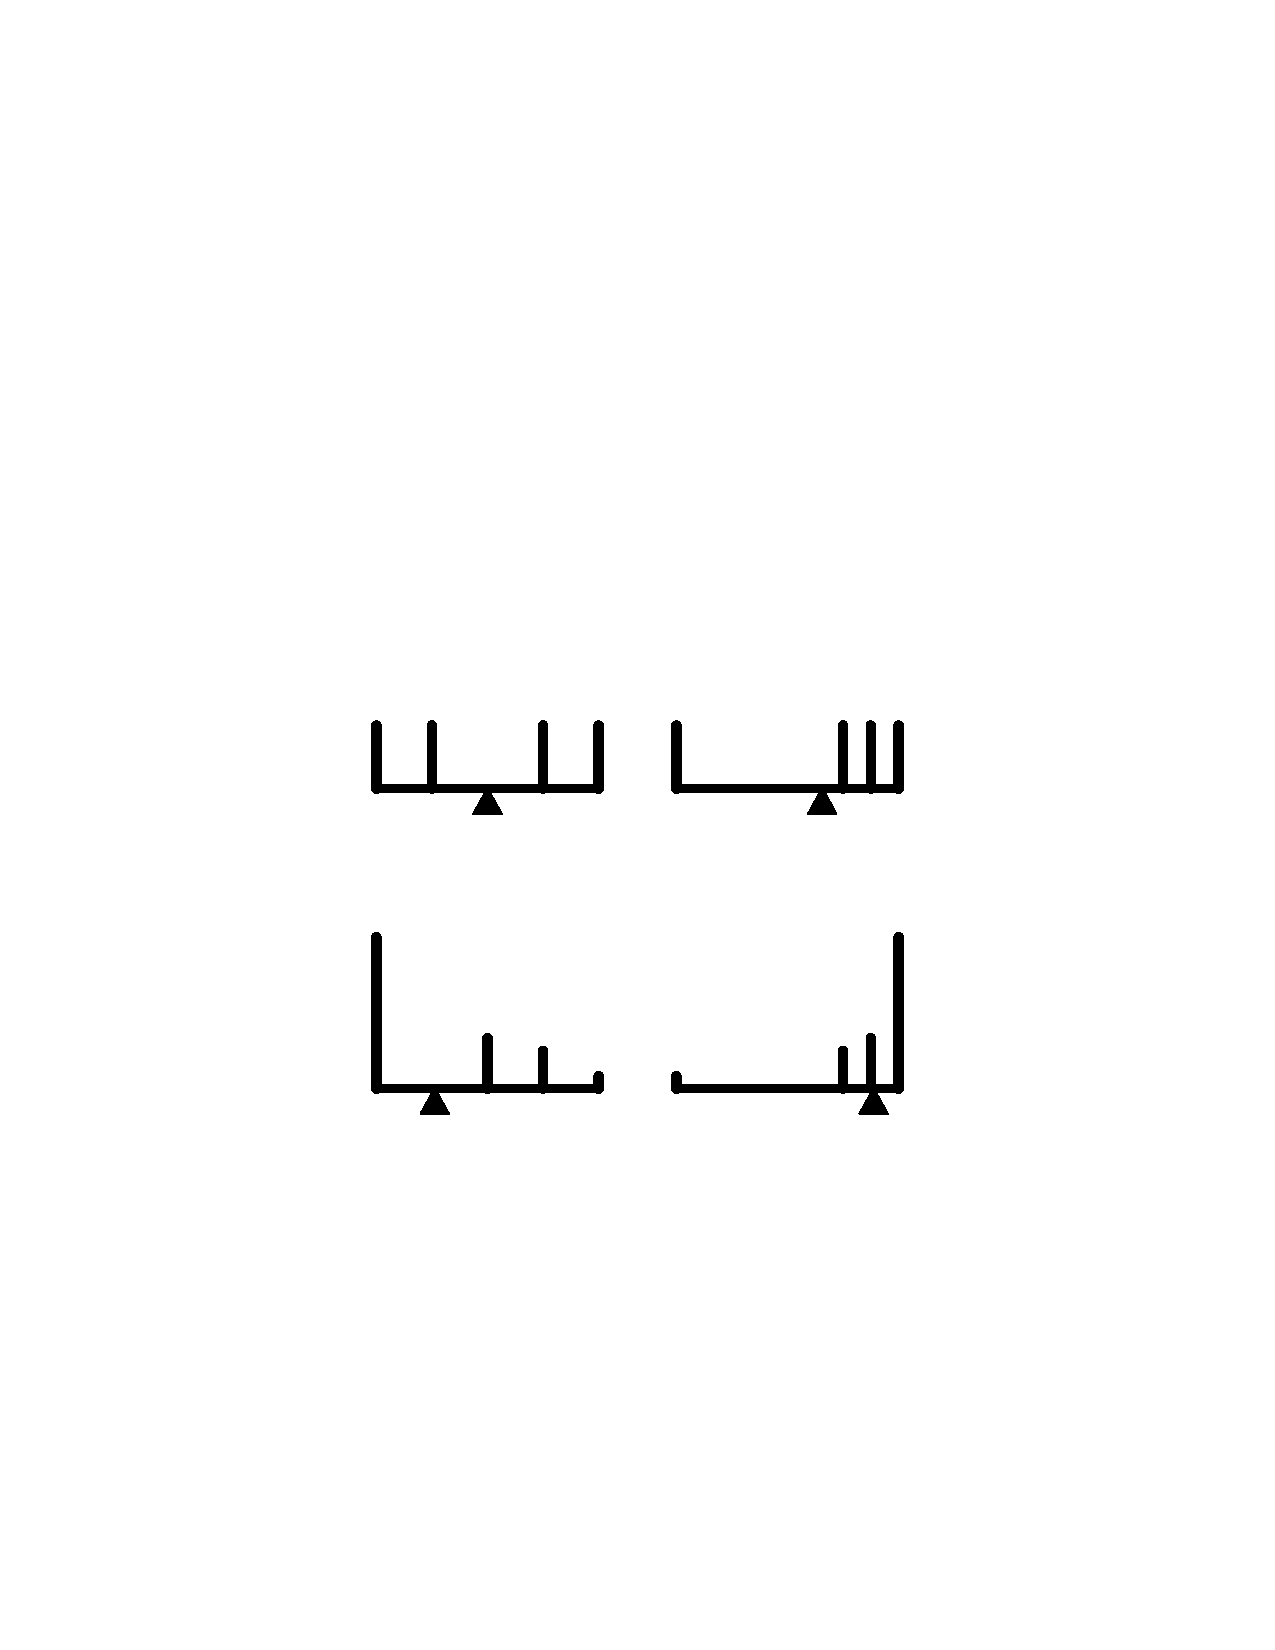
\includegraphics[width=3.5in]{expectation.pdf}
\end{frame}



\begin{frame}
  \frametitle{Example} 
  \begin{itemize}
  \item Suppose a coin is flipped and $X$ is declared $0$ or $1$ corresponding
    to a head or a tail, respectively
  \item What is the expected value of $X$? 
    $$
    E[X] = .5 \times 0 + .5 \times 1 = .5
    $$
  \item Note, if thought about geometrically, this answer is obvious; if two equal
    weights are spaced at 0 and 1, the center of mass will be $.5$
  \end{itemize}
\end{frame}

\begin{frame}\frametitle{Example} 
  \begin{itemize}
  \item Suppose that a die is tossed and $X$ is the number face up
  \item What is the expected value of $X$?
    $$
    E[X] = 1 \times \frac{1}{6} + 2 \times \frac{1}{6} +
    3 \times \frac{1}{6} + 4 \times \frac{1}{6} +
    5 \times \frac{1}{6} + 6 \times \frac{1}{6} = 3.5
    $$
  \item Again, the geometric argument makes this answer obvious without calculation.
  \end{itemize}
\end{frame}

\subsection{Continuous random variables}
\begin{frame}\frametitle{Continuous random variables}
  \begin{itemize}
  \item For a continuous random variable, $X$, with density, $f$, the expected
    value is defined as follows
    $$
    E[X] = \int_{-\infty}^\infty t f(t)dt
    $$
  \item This definition borrows from the definition of center of mass for
    a continuous body
  \end{itemize}
\end{frame}

\begin{frame}\frametitle{Example}
  \begin{itemize}
  \item   Consider a density where $f(x) = 1$ for $x$
    between zero and one
  \item (Is this a valid density?)
  \item Suppose that $X$ follows this density; what is its expected value? 
    $$
    E[X] = \int_{0}^{1} x dx = \left. \frac{x^2}{2} ~\right|_{0}^{1} = 1/2
    $$
  \end{itemize}
\end{frame}

\section{Rules about expected values}
\begin{frame}\frametitle{Rules about expected values}
  \begin{itemize}
  \item The expected value is a linear operator 
  \item If $a$ and $b$ are not random and $X$ and $Y$ 
    are two random variables then
    \begin{itemize}
    \item $E[aX + b] = a E[X] + b$
    \item $E[X + Y] = E[X] + E[Y]$
    \end{itemize}
  \item {\em In general} if $g$ is a function that is not linear,
    $$
    E[g(X)] \neq g(E[X])
    $$
  \item For example, in general, $E[X^2] \neq E[X]^2$ 
  \end{itemize}
\end{frame}

\begin{frame}\frametitle{Example}
  \begin{itemize}
  \item  You flip a coin, $X$ and simulate a uniform random number $Y$, what 
    is the expected value of their sum? 
    $$
    E[X + Y] = E[X] + E[Y] = .5 + .5 = 1
    $$ 
  \item Another example, you roll a coin twice. What is the expected value of
    the average? 
  \item Let $X_1$ and $X_2$ be the results of the two rolls
    $$
    E[(X_1 + X_2) / 2] = \frac{1}{2}(E[X_1] + E[X_2])
    = \frac{1}{2}(3.5 + 3.5) = 3.5
    $$
  \end{itemize}
\end{frame}


\begin{frame}\frametitle{Example}
  \begin{enumerate}
  \item Let $X_i$ for $i=1,\ldots,n$ be a collection of random
    variables, each from a distribution with mean $\mu$
  \item Calculate the expected value of the sample average of the $X_i$
  \end{enumerate}
  \begin{eqnarray*}
    E\left[ \frac{1}{n}\sum_{i=1}^n X_i\right]
    & = & \frac{1}{n} E\left[\sum_{i=1}^n X_i\right] \\
    & = & \frac{1}{n} \sum_{i=1}^n E\left[X_i\right] \\
    & = & \frac{1}{n} \sum_{i=1}^n \mu =  \mu.
  \end{eqnarray*}
\end{frame}

\begin{frame}
  \frametitle{Remark}
  \begin{itemize}
  \item Therefore, the expected value of the {\bf sample mean} is the {\bf
      population mean} that it's trying to estimate
  \item When the expected value of an estimator is what its trying to estimate,
    we say that the estimator is {\bf unbiased}
  \end{itemize}
\end{frame}


\section{Variances}
\begin{frame}\frametitle{The variance}
  \begin{itemize}
  \item The variance of a random variable is a measure of {\em spread}
  \item If $X$ is a random variable with mean $\mu$, the variance of 
    $X$ is defined as
    $$
    \Var(X) = E[(X - \mu)^2]
    $$
    the expected (squared) distance from the mean
  \item Densities with a higher variance are more spread out than
    densities with a lower variance
  \end{itemize}
\end{frame}

\begin{frame}
  \begin{itemize}
  \item Convenient computational form
    $$
    \Var(X) = E[X^2] - E[X]^2
    $$
  \item If $a$ is constant then $\Var(aX) = a^2 \Var(X)$
  \item The square root of the variance is called the {\bf standard deviation}
  \item The standard deviation has the same units as $X$
  \end{itemize}
\end{frame}


\begin{frame}\frametitle{Example}
  \begin{itemize}
  \item   What's the sample variance from the result of a toss of a die? 
    \begin{itemize}
    \item $E[X] = 3.5$ 
    \item $E[X^2] = 1 ^ 2 \times \frac{1}{6} + 2 ^ 2 \times \frac{1}{6} +
  3 ^ 2 \times \frac{1}{6} + 4 ^ 2 \times \frac{1}{6} +
  5 ^ 2 \times \frac{1}{6} + 6 ^ 2 \times \frac{1}{6} = 15.17$ 
    \end{itemize}
  \item $\Var(X) = E[X^2] - E[X]^2 \approx 2.92$
 \end{itemize}
\end{frame}

\begin{frame}\frametitle{Example}
  \begin{itemize}
  \item  What's the sample variance from the result of the toss of a coin
    with probability of heads (1) of $p$? 
    \begin{itemize}
    \item   $E[X] = 0 \times (1 - p) + 1 \times p = p$
    \item $E[X^2] = E[X] = p$ 
    \end{itemize}
  \item $\Var(X) = E[X^2] - E[X]^2 = p - p^2 = p(1 - p)$
  \end{itemize}
\end{frame}


\begin{frame}\frametitle{Example} 
  \begin{itemize}
  \item Suppose that a random variable is such that $0 \leq X \leq 1$ and $E[X] = p$
  \item Note $X^2 \leq X$ so that $E[X^2] \leq E[X] = p$
  \item $\Var(X) = E[X^2] - E[X]^2 \leq E[X] - E[X]^2 = p(1-p)$
  \item Therefore the Bernoulli variance is the largest possible for random variables bounded between $0$ and $1$
  \end{itemize}
\end{frame}

\section{Chebyshev's inequality}
\begin{frame}
\frametitle{Interpreting variances}
\begin{itemize}
  \item Chebyshev's inequality is useful for interpreting variances
  \item This inequality states that
    $$
    P(|X - \mu| \geq k\sigma) \leq \frac{1}{k^2}
    $$
  \item For example, the probability that a random variable lies beyond $k$
    standard deviations from its mean is less than $1/k^2$
    \begin{eqnarray*}
      2\sigma & \rightarrow & 25\% \\
      3\sigma & \rightarrow & 11\% \\
      4\sigma & \rightarrow &  6\% 
    \end{eqnarray*}
  \item Note this is only a bound; the actual probability might be
    quite a bit smaller
\end{itemize}
\end{frame}

\begin{frame} \frametitle{Proof of Chebyshev's inequality}
  \begin{eqnarray*}
    P(|X - \mu| > k\sigma) & = & \int_{\{x: |x-\mu| > k\sigma\}} f(x) dx \\
& \leq & \int_{\{x:|x -\mu| > k\sigma\}}\frac{(x - \mu)^2}{k^2\sigma^2} f(x) dx \\
& \leq & \int_{-\infty}^{\infty} \frac{(x - \mu)^2}{k^2\sigma^2} f(x) dx \\
& = & \frac{1}{k^2}
  \end{eqnarray*}
\end{frame}

\begin{frame} \frametitle{Example}
  \begin{itemize}
  \item IQs are often said to be distributed with a mean of $100$ and a sd of $15$
  \item What is the probability of a randomly drawn person having an IQ higher than
    $160$ or below $40$?
  \item Thus we want to know the probability of a person being more
    than $4$ standard deviations from the mean
  \item Thus Chebyshev's inequality suggests that this will be no larger than 6\%
  \item IQs distributions are often cited as being bell shaped, in which case this
    bound is very conservative
  \item The probability of a random draw from a bell curve being $4$
    standard deviations from the mean is on the order of $10^{-5}$ (one
    thousandth of one percent)
  \end{itemize}
\end{frame}

\begin{frame} \frametitle{Example}
  \begin{itemize}
  \item A popular buzz phrase in industrial quality control is
    Motorola's``Six Sigma'' whereby businesses are suggested to
    control extreme events or rare defective parts
  \item Chebyshev's inequality states that the probability of a ``Six
    Sigma'' event is less than $1/6^2 \approx 3\%$
  \item If a bell curve is assumed, the probability of a ``six sigma''
    event is on the oder of $10^{-9}$ (one ten millionth of a percent)
  \end{itemize}
\end{frame}
\end{document}
